\documentclass{beamer}

\usepackage{comment}
%\usetheme{default}
%\usetheme{AnnArbor}
%\usetheme{Antibes}
%\usetheme{Bergen}
%\usetheme{Berkeley}
%\usetheme{Berlin}
%\usetheme{Boadilla}
%\usetheme{CambridgeUS}
%\usetheme{Copenhagen}
%\usetheme{Darmstadt}
%\usetheme{Dresden}
%\usetheme{Frankfurt}
%\usetheme{Goettingen}
%\usetheme{Hannover}
%\usetheme{Ilmenau}
%\usetheme{JuanLesPins}
%\usetheme{Luebeck}
\usetheme{Madrid}
%\usetheme{Malmoe}
%\usetheme{Marburg}
%\usetheme{Montpellier}
%\usetheme{PaloAlto}
%\usetheme{Pittsburgh}
%\usetheme{Rochester}
%\usetheme{Singapore}
%\usetheme{Szeged}
%\usetheme{Warsaw}

% As well as themes, the Beamer class has a number of color themes
% for any slide theme. Uncomment each of these in turn to see how it
% changes the colors of your current slide theme.

%\usecolortheme{albatross}
%\usecolortheme{beaver}
%\usecolortheme{beetle}
%\usecolortheme{crane}
%\usecolortheme{dolphin}
%\usecolortheme{dove}
%\usecolortheme{fly}
%\usecolortheme{lily}
%\usecolortheme{orchid}
%\usecolortheme{rose}
%\usecolortheme{seagull}
%\usecolortheme{seahorse}
%\usecolortheme{whale}
%\usecolortheme{wolverine}


\usepackage[utf8]{inputenc}
\usepackage{default}
\usepackage{pgfpages}
\usepackage{bbm}
\usepackage{amsmath}
\usepackage{amssymb} 
\usepackage{amsthm}
\usepackage{epsfig}
\usepackage{natbib} 
\usepackage{apalike}
% \usepackage{floatrow}
\usepackage{wasysym}
\usepackage{mhchem}
\usepackage{xcolor}

\usepackage{multirow}
\usepackage{graphicx}
\usepackage{subfigure}
\usepackage{caption}
\usepackage{tikz}
\usepackage{array,caption,tabularx,booktabs}
\usepackage{pgfplots}
\usepackage{listings}
\captionsetup[figure]{labelformat=empty}
\usetikzlibrary{patterns}
\newcommand\arraybslash{\let\\\@arraycr}

\newenvironment{mysplit}%
  {\arraycolsep 0pt \begin{array}{l}}%
  {\end{array}}
  
\makeatletter 
\def\newblock{\beamer@newblock}
\makeatother

\makeatletter
\newcommand\resetstackedplots{
    \makeatletter
\pgfplots@stacked@isfirstplottrue
\makeatother
        \addplot [forget plot,draw=none] coordinates{(2,0) (4,0) (8,0) (16,0)};
    }

    \makeatletter
\newcommand{\thickhline}{%
    \noalign {\ifnum 0=`}\fi \hrule height 1pt
            \futurelet \reserved \xhline
}
\def\mystrut{\vphantom{hg}}

    
\definecolor{almond}{rgb}{0.94, 0.87, 0.8}
\definecolor{aliceblue}{rgb}{0.94, 0.97, 1.0}
\definecolor{atomictangerine}{rgb}{1.0, 0.6, 0.4}

\pgfplotsset{
    legend image with text/.style={
        legend image code/.code={%
            \node[anchor=center] at (0.3cm,0cm) {#1};
        }
    },
}


\usepackage{color}

\def\happensAt{\textsf{\footnotesize happensAt}}
\def\initially{\textsf{\footnotesize initially}}
\def\holdsAt{\textsf{\footnotesize holdsAt}}
\def\holdsFor{\textsf{\footnotesize holdsFor}}
\def\initiatedAt{\textsf{\footnotesize initiatedAt}}
\def\terminatedAt{\textsf{\footnotesize terminatedAt}}
\def\broken{\textsf{\footnotesize broken}}
\def\startE{\textsf{\footnotesize start}}
\def\endE{\textsf{\footnotesize end}}

\def\unionall{\textsf{\footnotesize union\_all}}
\def\intersectall{\textsf{\footnotesize intersect\_all}}
\def\complementall{\textsf{\footnotesize relative\_complement\_all}}
\def\abscomplementall{\textsf{\footnotesize complement\_all}}

\def\nbf{\textsf{\footnotesize not}}
\def\true{\textsf{\footnotesize true}}
\def\false{\textsf{\footnotesize false}}
\def\since{\textsf{\footnotesize since}}

\def\rtec{$\mathit{RTEC}$}
\DeclareMathOperator{\val}{=}  % for p=v atoms
\DeclareMathOperator{\notval}{\neq}  % for p=v atoms


\title[RTEC]{Introduction to Run-Time Event Calculus} % The short title appears at the bottom of every slide, the full title is only on the title page

\author[]{Manos Pitsikalis, Alexander Artikis} % Your name
\institute[NCSR `Demokritos'] % Your institution as it will appear on the bottom of every slide, may be shorthand to save space
{
Institute of Informatics \& Telecommunications\\
NCSR `Demokritos'\\% Your institution for the title page
\medskip
\textit{manospits@iit.demokritos.gr} % Your email address
}
\date{\today} %

\begin{document}

\begin{frame}
\titlepage % Print the title page as the first slide
\end{frame}

%======================================

\begin{frame}[fragile]
 \frametitle{RTEC: Manual}
 The RTEC \textbf{manual} contains detailed instructions for the use of RTEC. If you have more questions refer to the \textbf{manual} ...or ask me (manospits@iit.demokritos.gr).\\
\pause
\hfill \\
What is the main file of RTEC?
\begin{lstlisting}[basicstyle=\tiny,]
 -- src
    |-- compiler.prolog
    |-- inputModule.prolog
    |-- processEvents.prolog
    |-- processSDFluents.prolog
    |-- processSimpleFluents.prolog
    |-- RTEC.prolog
    |-- utilities
        |-- amalgamate-periods.prolog
        |-- interval-manipulation.prolog
\end{lstlisting}

\pause
Answer: `RTEC.prolog'
\end{frame}


%======================================

\begin{frame}
\frametitle{Composite Event Recognition}
\centering
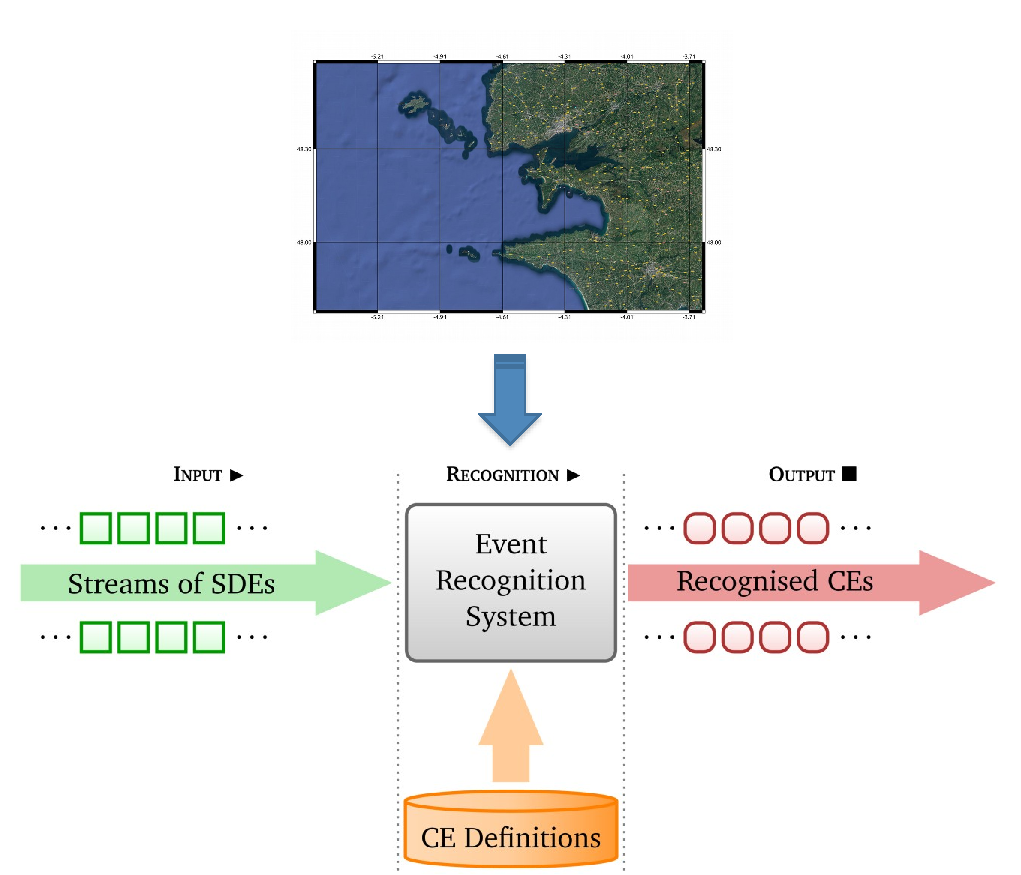
\includegraphics[width=8cm]{./graphics/cer-mar}
\end{frame}

%======================================

\begin{frame}
   \frametitle{Event Calculus}


\begin{itemize}
\item A \textbf{logic programming language} for representing and reasoning about events and their effects.
\pause
\item Key components:
\begin{itemize}
  \item \textbf{event} (typically instantaneous).
  \item \textbf{fluent}: a property that may have different values at different points in time.
\end{itemize}
\pause
\item Built-in representation of \textbf{inertia}:
\begin{itemize}
  \item $F \val V$ holds at a particular time-point if $F \val V$ has been \emph{initiated} by an event at some earlier time-point, and not \emph{terminated} by another event in the meantime.
\end{itemize}

\end{itemize}

\end{frame}

%======================================

\begin{frame}[fragile]
\frametitle{Event Recognition Engine : RTEC}
\begin{itemize}
  
\item \textbf{Event Calculus for Run-Time reasoning} (\rtec) is the implementation of the Event Calculus designed to efficiently perform composite event recognition. 
\item \rtec\  recognizes from a stream of low level events the maximal intervals of durative composite events, or timepoints respectively for instantaneous events.
\end{itemize}
\end{frame}

%======================================

\begin{frame}
   \frametitle{RTEC : Predicates}
\begin{table}[t]
\scriptsize
\begin{center}
\renewcommand{\arraystretch}{0.9}
\setlength\tabcolsep{4.6pt}
\begin{tabular}{ll}
\hline\noalign{\smallskip}
\multicolumn{1}{c}{\textbf{Predicate}} & \multicolumn{1}{c}{\textbf{Meaning}}  \\
\noalign{\smallskip}
\hline
\noalign{\smallskip}
\happensAt$(E, T)$ & {\scriptsize Event $E$ occurs at time $T$}  \\[5pt]

\initiatedAt$(F \val V, T)$ & {\scriptsize At time $T$ a period of time for which}\\
								     & {\scriptsize $F\val V$ is initiated} \\[5pt]

\terminatedAt$(F \val V, T)$ & {\scriptsize At time $T$ a period of time for which} \\
									 & {\scriptsize $F\val V$ is terminated} \\[5pt]

\holdsFor$(F \val V, I)$ & {\scriptsize $I$ is the list of the maximal intervals} \\
                           					  & {\scriptsize for which $F\val V$ holds continuously} \\[5pt]

\holdsAt$(F \val V, T)$ & {\scriptsize The value of fluent $F$ is $V$ at time $T$} \\[5pt]

\unionall$\mathit{([J_1,\dots,J_n],\ I)}$ & $I\val (J_1\cup\ldots\cup J_n)$ \\[5pt]

\intersectall$\mathit{([J_1,\dots,J_n],\ I)}$ &  $I\val (J_1\cap\ldots\cap J_n)$\\[5pt]

\complementall &  $I\val I' \setminus (J_1\cup\ldots\cup J_n)$\\
$\mathit{\footnotesize (I',\ [J_1,\dots,J_n],\ I)}$ & \\
\hline
\end{tabular}
\end{center}
\end{table}
\end{frame}

%======================================

\begin{frame}[fragile]
\frametitle{RTEC: Fluents}
Fluents in RTEC can be either \textbf{simple} or \textbf{statically determined fluents}.
\begin{itemize}
  
\item \textbf{Simple fluents} are defined by specifying the initiation and termination conditions with the use of $\mathit{\initiatedAt}$ and $\mathit{\terminatedAt}$ predicates. 
\item \textbf{Statically determined fluents} are defined with the use of $\mathit{\holdsFor}$ rules.

\end{itemize}
\end{frame}

%======================================

\begin{frame}[fragile]
\frametitle{Simple Fluents: Example}
A vessel could be considered stopped when it has a speed value less than 0.5 knots.

\begin{align*} 
\footnotesize
        \begin{mysplit}
            \initiatedAt\mathit{(stopped(Vessel) \val \true,\ T) \leftarrow}\\
            \quad    \happensAt\mathit{(velocity(Vessel,Speed,Heading,CoG),T)},\\
            \quad    \mathit{Speed < 0.5}.\\
            \terminatedAt\mathit{(stopped(Vessel) \val \_PortStatus,\ T) \leftarrow}\\
            \quad    \happensAt\mathit{(velocity(Vessel,Speed,Heading,CoG),T)},\\
            \quad    \mathit{Speed >= 0.5}.\\
        \end{mysplit}
    \end{align*} 
\end{frame}

%======================================

\begin{frame}[fragile]
\frametitle{Statically Determined Fluents: Example}
A `naive' definition of vessels sailing with travel speed is the following:
\begin{align*} 
\footnotesize
        \begin{mysplit}
            \holdsFor\mathit{(travelSpeed(Vessel) \val \true,\ I) \leftarrow}\\
            \quad    \holdsFor\mathit{(underWay(Vessel),I_u)}\\
            \quad    \holdsFor\mathit{(lowSpeed(Vessel),I_l)}\\            
            \quad    \complementall{(I_u,[I_l],I)}.\\
        \end{mysplit}
    \end{align*} 
\end{frame}

%======================================

\begin{frame}[fragile]
\frametitle{RTEC recognition parameters}
RTEC performs recognition using a window mechanism i.e., working memory.
\begin{itemize}
\item \textbf{Step}: CE recognition takes place at query times $Q_1,Q_2,\ldots,Q_i,\ldots,Q_n$\ where $Q_i- Q_{i-1} = Step$\ is a constant value.
\item \textbf{WM}: At each $Q_i$ RTEC computes the maximal intervals of CEs using input events that fall within the interval $(Q_{i-WM},Q_{i}]$. Input events that occur before $Q_{i-WM}$ are discarded.
\end{itemize}
\end{frame}

%=====================================

\begin{frame}[fragile]
\frametitle{RTEC: Windows}
\begin{center}
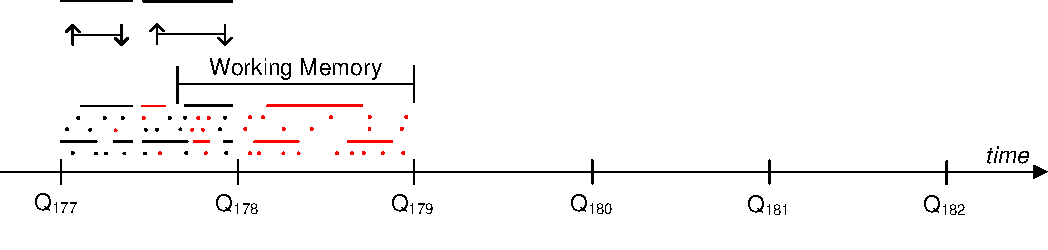
\includegraphics[width=0.8\linewidth]{./graphics/windows1.pdf}
\pause

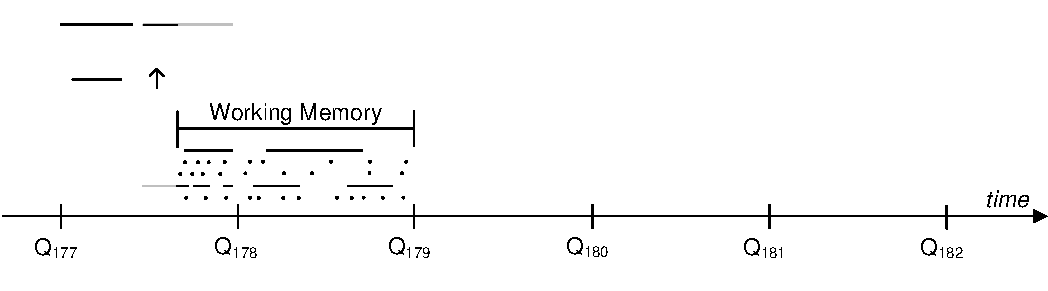
\includegraphics[width=0.8\linewidth]{./graphics/windows2.pdf}
\pause

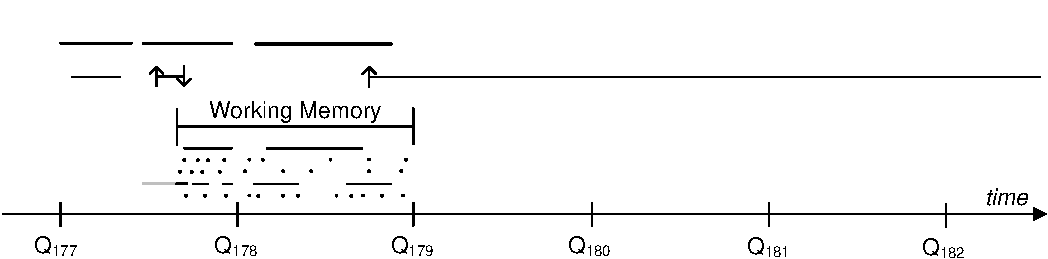
\includegraphics[width=0.8\linewidth]{./graphics/windows3.pdf}

\end{center}
\end{frame}

%======================================

\begin{frame}[fragile]
\frametitle{RTEC: Main files}
\begin{itemize}
 \item A \textbf{patterns file} that contains rules written in the language of RTEC.
 \item A \textbf{declarations file} that contains the appropriate declarations for all the input and output entities. 
 \item The \textbf{`RTEC.prolog'} is the main file of the RTEC implementation. It is required both for the compilation of rules and the recognition process.
 \item The \textbf{'continuousQueries.prolog'} file is used for performing event recognition.
\end{itemize}
\end{frame}

%======================================

\begin{frame}[fragile]
\frametitle{RTEC: Patterns file}

\begin{lstlisting}[language=Prolog, basicstyle=\tiny,]
initiatedAt(stopped(Vessel)=true,T):-
    happensAt(velocity(Vessel,Speed,_CoG,_TrHeading),T),
    Speed < 0.5.  %knots

terminatedAt(stopped(Vessel)=true,T):-
    happensAt(velocity(Vessel,Speed,_CoG,_TrHeading),T),
    Speed >= 0.5. %knots

initiatedAt(lowSpeed(Vessel)=true,T):-
    happensAt(velocity(Vessel,Speed,_CoG,_TrHeading),T),
    Speed >= 0.5,  %knots
    Speed < 5.0.   %knots

terminatedAt(lowSpeed(Vessel)=true,T):-
    happensAt(velocity(Vessel,Speed,_CoG,_TrHeading),T),
    Speed < 0.5.  %knots

terminatedAt(lowSpeed(Vessel)=true,T):-
    happensAt(velocity(Vessel,Speed,_CoG,_TrHeading),T),
    Speed >= 5.0.  %knots
\end{lstlisting}
\end{frame}

%======================================

\begin{frame}[fragile]
\frametitle{RTEC: Declarations file}
\footnotesize
\begin{itemize}
\item For each entity state if it is input or output (simple fluents are by definition output entities), and state its index.
\begin{lstlisting}[language=Prolog, basicstyle=\tiny,]
event(velocity(_,_,_,_)).
inputEntity(velocity(_,_,_,_)).
index(velocity(Vessel,_,_,_), Vessel).
 ...
simpleFluent(stopped(_) = true).
outputEntity(stopped(_) = true).
index(stopped(Vessel) = true, Vessel).
 ...
sDFluent(travelSpeed(_)=true).
outputEntity(travelSpeed(_)=true).
index(travelSpeed(Vessel)=true, Vessel).
\end{lstlisting}
\pause
\item Declare the groundings of the fluents and output entities/events.
\begin{lstlisting}[language=Prolog, basicstyle=\tiny,]
grounding(stopped(Vessel) = true)     :- vessel(Vessel).
 ...
grounding(travelSpeed(Vessel) = true) :- vessel(Vessel).
\end{lstlisting}
\pause
\item A caching order should be defined for all output entities. Caching order is the order in which output entities are processed.
\begin{lstlisting}[language=Prolog, basicstyle=\tiny,]
cachingOrder(stopped(_) = true).
 ...
cachingOrder(travelSpeed(_) = true).
\end{lstlisting}
\end{itemize}
\end{frame}

%======================================

\begin{frame}[fragile]
\frametitle{RTEC: Preparation}
\footnotesize
In order to perform event recognition with RTEC, first you must compile the rules...
\begin{lstlisting}[language=Prolog, basicstyle=\tiny,]
% open yap prolog
['RTEC.prolog']. %load RTEC file
compileEventDescription('./declarations.prolog',      % path to declarations file
                        './patterns.prolog',          % path to patterns file
                        './compiled_patterns.prolog').% path to compiled patterns
\end{lstlisting}
\pause
...create a dataset in the appropriate form...
\begin{lstlisting}[language=Prolog, basicstyle=\tiny,]
%Event|T|T|Arg1|...|ArgN
coord|1455926402|1455926402|227091000|-4.478240000|48.383200000
%Fluent|Te|Ts|Te|Value|Arg1|...|ArgN
proximity|1455926423|1455926423|1455926423|true|227091000|227574020
\end{lstlisting}
\pause
...create a file with the grounding domains...
\begin{lstlisting}[language=Prolog, basicstyle=\tiny,]
vessel(227091000).
vessel(227574020).
 ...
\end{lstlisting}
then...
\end{frame}

%======================================

\begin{frame}[fragile]
\frametitle{RTEC: Recognition}
\footnotesize
Load the necessary files and perform recognition.
\begin{lstlisting}[language=Prolog, basicstyle=\tiny,]
['continuousQueries.prolog']
['declarations.prolog'].
['compiled_patterns.prolog'].
['vessels.prolog'].

% continuousER(
%   DatasetFile, DatasetFile is the input dataset file
%   OutputFile,  OutputFile records recognised CEs
%   TimesFile,   TimesFile records the event recognition times,
%   InputFile,   InputFile records the number of input events per window,
%   InitPoint,   InitPoint is where recognition starts,
%   LastTime,    LastTime is where recognition ends,
%   WM,          WM is the window size,
%   Step         Step is the recognition step.
%  )

continuousER('dataset.txt','recognised_CEs.txt',
              'stats_times.txt','stats_input.txt',
              1455926402,1456358403,86400,86400).
\end{lstlisting}

\end{frame}

%======================================
\begin{comment}
\begin{frame}
 \frametitle{Stream preprocessing: architecture}
 \begin{center}
  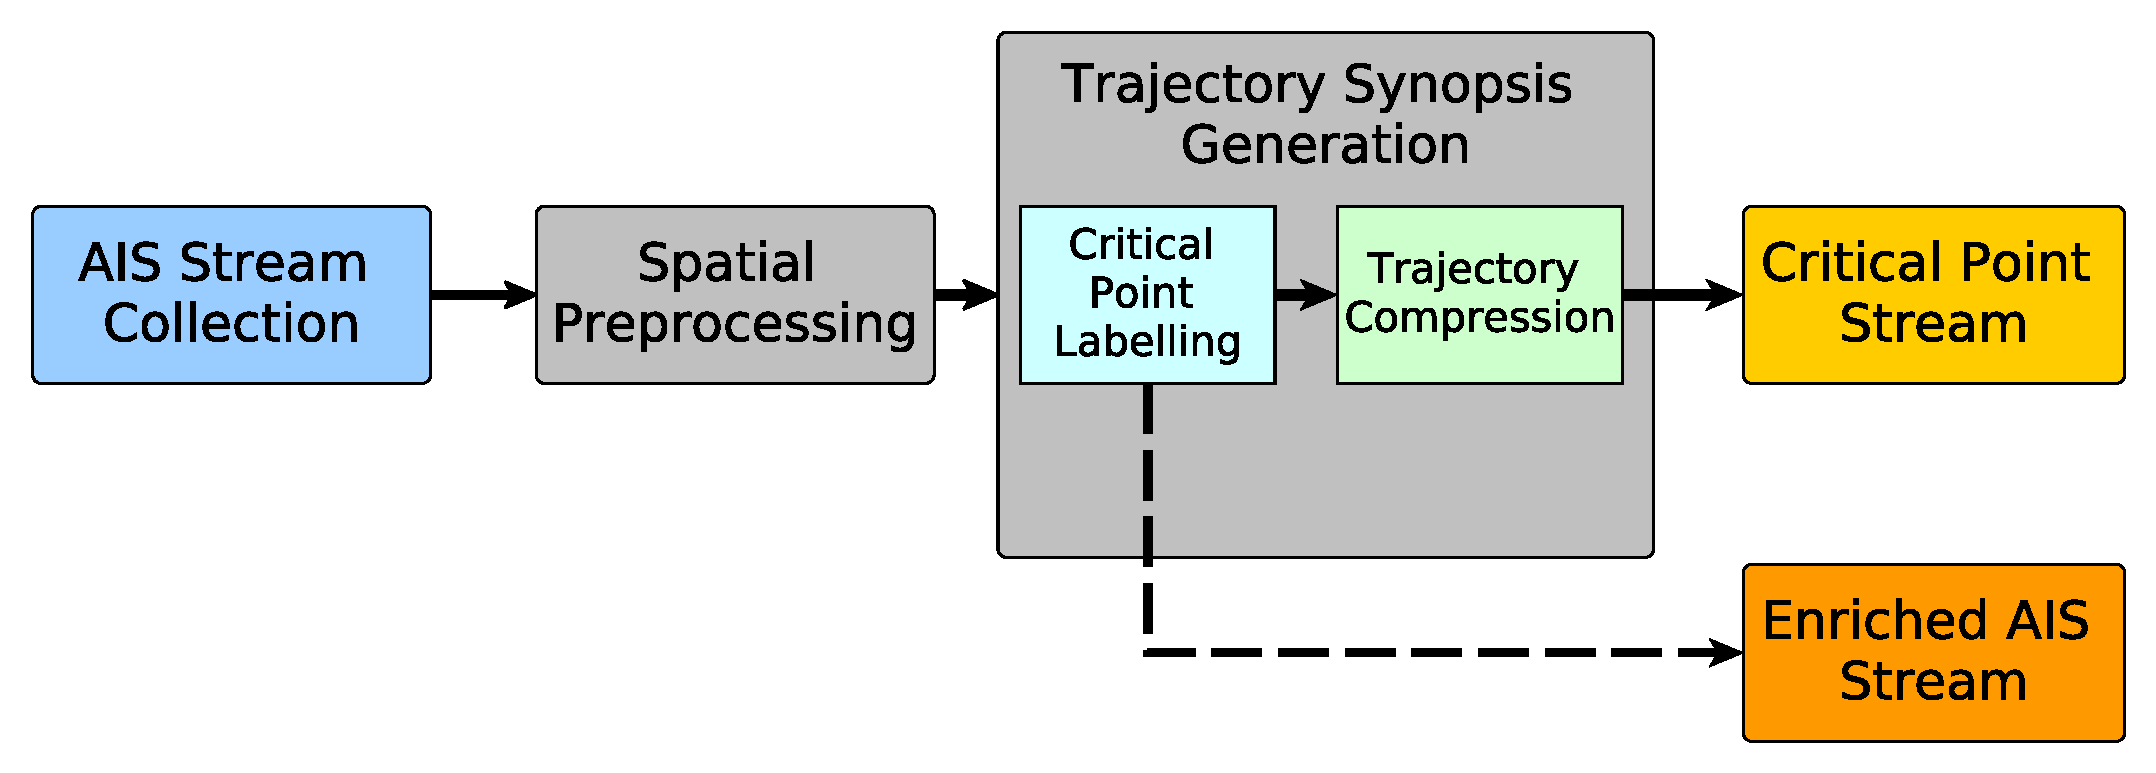
\includegraphics[width=0.8\linewidth]{./graphics/streams.pdf}
 \end{center}
\end{frame}

%======================================

\begin{frame}
 \frametitle{Stream preprocessing: components}
 \begin{itemize}
  \item \textbf{Spatial preprocessing}: During the spatial link discovery step spatial events, linking vessels with areas or vessels with other vessels are detected.
  \item \textbf{Trajectory Synopses Generation}: During the tajectory synopses generation step, only the most important transmitted positions or as we call them `critical points',  are identified, annotated and retained.
 \end{itemize}
\end{frame}

%=====================================

 \begin{frame}
 \frametitle{Stream preprocessing: events}
\begin{table}[t]
\scriptsize
\begin{center}
\renewcommand{\arraystretch}{0.9}
\setlength\tabcolsep{4.6pt}
\begin{tabular}{ll}
\hline\noalign{\smallskip}
\multicolumn{1}{c}{\textbf{Event}} & \multicolumn{1}{c}{\textbf{Meaning}}  \\
\noalign{\smallskip}
\hline
\hline
\noalign{\smallskip}
$\mathit{entersArea(V,AreaType)}$ & {\scriptsize A vessel $V$ enters an area of $\mathit{AreaType}$}  \\[5pt]
$\mathit{leavesArea(V,AreaType)}$ & {\scriptsize A vessel $V$ leaves an area of $\mathit{AreaType}$}  \\[5pt]
$\mathit{proximity(V_1,V_2)=true}$ & {\scriptsize Two vessels $V_1,V_2$ are within 100 m} \\[5pt]
\hline\\[-2pt]
$\mathit{gap\_start(V)}$ & {\scriptsize A communication gap starts for vessel $V$}  \\[5pt]
$\mathit{gap\_end(V)}$ & {\scriptsize A communication gap ends for vessel $V$}  \\[5pt]
$\mathit{slow\_motion\_start(V)}$ & {\scriptsize A vessel $V$ starts sailing with low speed}  \\[5pt]
$\mathit{slow\_motion\_end(V)}$ & {\scriptsize A vessel $V$ stops sailing with low speed}  \\[5pt]
$\mathit{change\_in\_speed\_start(V)}$ & {\scriptsize A vessel $V$ starts changing speed}  \\[5pt]
$\mathit{change\_in\_speed\_end(V)}$ & {\scriptsize A vessel $V$ stops changing speed}  \\[5pt]
$\mathit{change\_in\_heading(v)}$ & {\scriptsize A vessel $V$ changes course }\\
\hline
\end{tabular}
\end{center}
\end{table}
\end{frame}

%===================================
\begin{frame}
 \frametitle{Stream preprocessing: parameters}
  \begin{table}
    \footnotesize
    \begin{center}
        \renewcommand{\arraystretch}{0.9}
        \setlength\tabcolsep{3.6pt}
        \begin{tabular}{lc}
            \hline\noalign{\smallskip}
            \toprule
            Parameter & Value             \\ \midrule
            Minimum speed $\mathit{v_{min}}$ (knots) for asserting movement (stopped) & 0.5\\[3pt]
            Maximum speed $\mathit{v_\theta}$ (knots) for asserting slow motion & 5\\[3pt]
            Minimum rate $\mathit{\alpha}$ for asserting speed change between locations & 0.25\\[3pt]
            Minimum period $\mathit{\Delta T}$ (seconds) for asserting communication gap & 1800\\[3pt]
            Angle threshold $\mathit{\Delta\theta}$ (degrees)for asserting change in heading & 4 \\
            \bottomrule
        \end{tabular}
    \end{center}
\end{table}

\end{frame}

%====================================

\begin{frame}
 \frametitle{Pre-processed Brest dataset}
 \begin{itemize}
  \item \textbf{Enriched stream of the Brest dataset}: link...
 \end{itemize}

\end{frame}

%====================================

\begin{frame}
 \frametitle{Bibliography}
 \begin{itemize}
  \item Alexander Artikis, Marek J. Sergot, and Georgios Paliouras. 2015. An Event
Calculus for Event Recognition. IEEE Trans. Knowl. Data Eng. 27, 4 (2015),
895–908.
  \item Robert A. Kowalski and Marek J. Sergot. 1986. A Logic-based Calculus of
Events. New Generation Comput. 4, 1 (1986), 67–95.
  \item Harris Georgiou, Sophia Karagiorgou, Kostas Patroumpas, Nikos Pelekis, Pet-
ros Petrou, Stylianos Sideridis, Eugenia Stoufi, and Yannis Theodoridis. 2017.
datACRON: D2.1 Cross-streaming, real-time detection of moving object tra-
jectories. (2017). 
 \end{itemize}

\end{frame}
\end{comment}

\end{document}
